\section{A contraction-certified execution-tracking construction}
\label{app:contraction-example}
This constructed servo demonstrates how the sampled conditions produce a
useful, independently reproducible recovery envelope. It is not an additional
VLA evaluation. The certificate concerns execution tracking under a common
command reference, not contraction of the augmented adaptive system or a
contact-rich policy.

\paragraph{Plant and exact metric.}
At $20$\,ms command intervals, let $\xi_k\in\mathbb R^2$ be position in meters,
$c_k=(.06\sin(.6t_k),\,.03\cos(.4t_k))^\top$ a supplied position reference,
and $t_k=.02k$. Define
\begin{equation}
\begin{aligned}
\xi_{k+1}&=A\xi_k+u_k+f_k,&
\xi_{k+1}^{\rm nom}&=A\xi_{k}^{\rm nom}+a_k,\\
a_k&=(I-A)c_k,&
u_k&=\operatorname{clip}_{[-.025,.025]^2}
       (a_k-D\fhat_{\tau_k}).
\end{aligned}
\label{eq:construction-plant}
\end{equation}
\begin{equation}
P=\operatorname{diag}(1,4),\qquad
A=.92P^{-1/2}\operatorname{Rot}(.04)P^{1/2}.
\label{eq:construction-metric}
\end{equation}
Here $A$ represents the nominal robot with its execution controller, not an
uncontrolled integrator. The supplied command in Theorem~\ref{thm:tube} is
$a_k$; the nominal physical copy receives this
same sequence. The position target $c_k$ is not itself the nominal response
$\xi_{k}^{\rm nom}$. Commands and faults are additive position increments in meters.
Orthogonality of $\operatorname{Rot}$ gives $A^\top PA=.92^2P$ globally.
Thus $M_{c,k}=P$, $X_k=\|\xi_k-\xi_{k}^{\rm nom}\|_P$,
$\lambda_k^{\rm exec}=.92$, and $L_k=\sqrt{\lambda_{\max}(P)}=2$ satisfy
the sufficient smooth-mode condition in Eq.~\eqref{eq:sampled-metric}, hence
Eq.~\eqref{eq:sampled-contraction}, and the input bound for every state.
These constants are analytical; no trajectory fit or sampled Jacobian search
is used. The equivalent nominal forgetting rate is
$-\log(.92)/.02=4.169\,\mathrm{s}^{-1}$.

\paragraph{Causal proprioception and imperfect centering.}
After command $k$, the measured execution increment is
$v_k=\xi_{k+1}-A\xi_k=u_k+f_k$. A seven-tap proprioceptive filter and its healthy
predictor produce
\begin{equation}
\begin{aligned}
y_k&=S\sum_{\ell=0}^6h_\ell v_{k-\ell}+Sb,&
\widehat y_k&=S\sum_{\ell=0}^6h_\ell u_{k-\ell},\\
z_k&=S^{-1}(y_k-\widehat y_k)
 =\sum_{\ell=0}^6h_\ell f_{k-\ell}+b.
\end{aligned}
\label{eq:construction-sensor}
\end{equation}
where $S=\operatorname{diag}(1,.7)$,
$h=(.40,.25,.15,.10,.05,.03,.02)$, and
$b=(.0003,-.0002)^\top$\,m is unremoved sensor-centering bias.
The fault is zero before $k=50$ and
$f_k=(.006,.0025)^\top$\,m thereafter. Prehistory has $u_k=v_k=f_k=0$ for
$k<0$. Therefore the onset contribution to $w_k=z_k-f_k$ is exactly
$-\sum_{\ell=j+1}^6h_\ell f_{50}$ at $k=50+j$, $0\le j\le6$;
it vanishes in response $k=56$, acquired at $1.14$\,s, which is $120$\,ms
after the first post-fault response. Observations are plotted at their
acquisition times $t_{k+1}$.
The estimator uses measured $z_k$, never injected fault truth.

\paragraph{Actual update, projection, and application.}
We apply Eqs.~\eqref{eq:legacy} and~\eqref{eq:innovation} with
$P_r=I_2$, $\gamma=.08$, $\rho=.015$\,m, $\delta=.0008$\,m, and
coordinatewise projection onto $\mathcal C=[-.015,.015]^2$\,m. The innovation
gain depends on the current estimate exactly as in Eq.~\eqref{eq:innovation}.
Both coordinates are estimated in every adaptive condition. Full correction
uses $D=I_2$; the insufficient-support condition uses
$D=\operatorname{diag}(1,0)$ and the same innovation estimator. The frozen
condition has $D=0$ and no updates.
All states and estimates start at zero. Across the $600$ commands,
$\chi_k=0$ for $65\le k<100$ and whenever $k\bmod10=9$, and is one otherwise.
These are preset clock-based missed updates, independent of fault truth.
A five-command application chunk uses
$\tau_k=\max\{0,5\lfloor k/5\rfloor-2\}$; snapshot age is at most six steps.
An estimate updated after response $k$ first exists at index $k+1$.
Projection and command clipping are implemented separately. Convexity keeps
the update targets and estimates inside $\mathcal C$; furthermore
$|I-A|(.06,.03)^\top+.015\mathbf1<(.02206,.01854)^\top<.025\mathbf1$.
Neither projection nor command clipping activates, even if the construction
is continued indefinitely, so $\zeta_k=0$.

\begin{figure}[t]
\centering
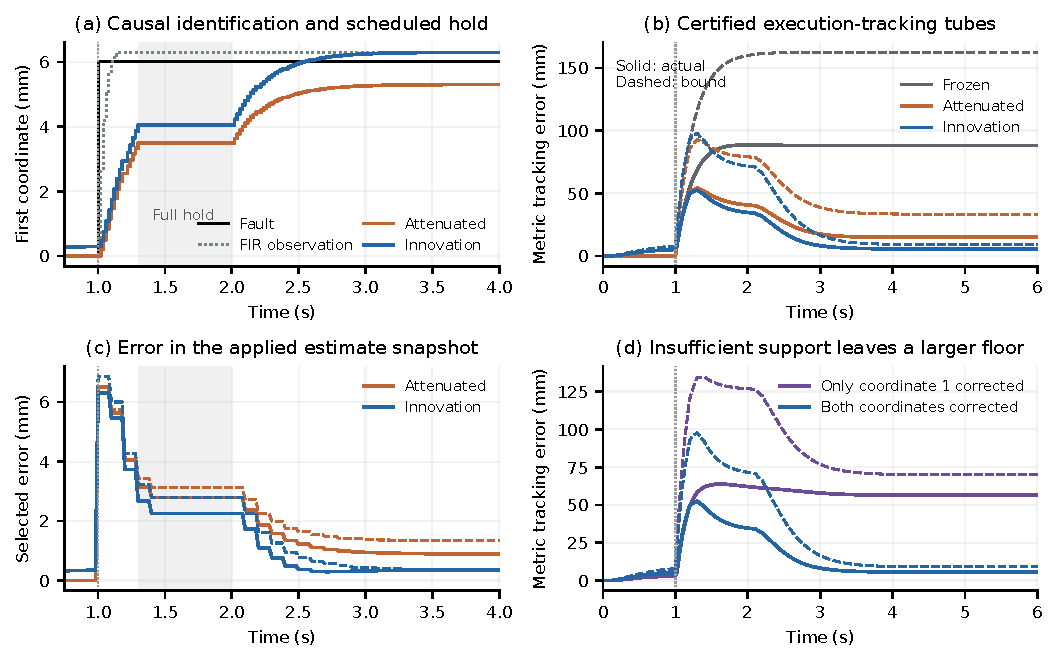
\includegraphics[width=\linewidth]{fig_contraction_tracking.pdf}
\caption{Constructed execution servo with a globally verified constant metric.
Solid curves are realized errors or estimates; dashed curves in (b)--(d)
are analytically propagated bounds. Shading denotes full-update holds.
The FIR delays fault observation, and chunk snapshots delay application.
Persistent centering bias gives a nonzero innovation floor; attenuation and
missing correction support produce larger floors. Every bound is checked
over the full $12$\,s rollout; panels show the recovery interval.}
\label{fig:contraction-tracking}
\end{figure}

\paragraph{Bound propagation and interpretation.}
The prescribed fault history and centering bias give the unfitted bound
\begin{equation}
\epsilon_k^D=\left\|D\sum_\ell h_\ell(f_{k-\ell}-f_k)\right\|+\|Db\|.
\end{equation}
Use the exact selected fault increments in Proposition~\ref{thm:estimator}.
Starting from $B_0^D=R_0=0$, propagate the actual-family bound,
the snapshot minimum in Eq.~\eqref{eq:applied-delay}, and
\begin{equation}
R_{k+1}=.92R_k+2\bigl(\|(I-D)f_k\|+B_k^{D,\rm app}+\|\zeta_k\|\bigr).
\label{eq:construction-tube}
\end{equation}
These are valid model-based bounds for this prescribed construction; fault
truth is used only to evaluate their inputs, not by the adaptation law.
The global metric removes a domain-containment restriction for this servo.

For a constant post-onset observation, the full-correction estimate limits
are $\fhat_\infty=s_\infty(f+b)$ for attenuation and
$\fhat_\infty=f+b$ for innovation, where $s_\infty=.841807$.
The clock retains infinitely many active updates when extended periodically,
and the box and $\|S\|=1$ give
$\alpha_k\ge.08/[1+(2\sqrt2)^2]=.008\overline8$ on active updates.
Finite snapshot age does not change these limits.
The exact state-error limit is
$\|(I-A)^{-1}(f-D\fhat_\infty)\|_P$.
Its values, followed by the propagated envelope limits, are
$88.03/162.50$\,mm (frozen), $14.94/33.29$\,mm (attenuated),
$5.64/9.01$\,mm (innovation), and $56.46/70.00$\,mm (restricted support).
The same fixed centering bias also causes a small healthy innovation drift
before fault onset, visible in Figure~\ref{fig:contraction-tracking}b.
The construction therefore illustrates useful recovery bounds without
equating contraction with unbiased identification or complete authority.

The released \code{audit/verify\_contraction\_tracking.py} reproduces the
figure, full trajectories, and assertions for the metric identity, causal
observation, selected estimate error, applied snapshot, and state envelope.
All assertions pass at absolute tolerance $10^{-11}$ (meters for error
inequalities); the metric identity's numerical
spectral residual is $4.1\times10^{-18}$. Numerical checks validate this
implementation of the analytical certificate; they do not certify any VLA
rollout or establish full adaptive-system incremental contraction.
